\documentclass[10pt]{article}
\usepackage{braket}
\usepackage{algorithm}
\usepackage{algpseudocode}
\usepackage{soul}
\usepackage{float}
\usepackage{tabularx}
\usepackage{mathtools}
\usepackage{amsmath, amssymb, amsthm}
\usepackage{tikz}
\usetikzlibrary{arrows}
\usetikzlibrary{decorations.text}
\usepackage{enumitem}
\usepackage{geometry}
\usepackage{fancyhdr}
\usepackage{titlesec}
\usepackage{xltabular}
\usepackage{color}
\usepackage{hyperref}
\geometry{margin=1in}

\pagestyle{fancy}
\fancyhf{}
\cfoot{\thepage}
\title{SFWRENG 3DX4 - Pre-lab 3}
\author{Matthew Farah, \href{mailto:farahm11@mcmaster.ca}{$\langle$farahm11@mcmaster.ca$\rangle$}, 400468251}
\date{\today}

\hypersetup{
	colorlinks=true,
	linkcolor=blue,
	filecolor=magenta,
	urlcolor=blue,
	citecolor=blue,
	anchorcolor=blue
}

\fancyhead{}
\fancyhead[L]{Matthew Farah, \href{mailto:farahm11@mcmaster.ca}{$\langle$farahm11@mcmaster.ca$\rangle$}, 400468251}
\fancyhead[R]{SFWRENG 3DX4 - Pre-lab 3}

\AtBeginEnvironment{align}{\setcounter{equation}{0}}

\newcommand{\comment}[1]{\parbox[t]{0.45\textwidth}{\raggedright #1}}

\setlength{\parindent}{0cm}

\setcounter{tocdepth}{3}
\hypersetup{bookmarksopen=true, bookmarksopenlevel=2, bookmarksdepth=3}

\newcounter{question}
\renewcommand{\thequestion}{\arabic{question}}

\newenvironment{question}{
	\refstepcounter{question}
	\phantomsection
	\addcontentsline{toc}{section}{\protect{\large{Question \thequestion}}}
	\vspace{1em}
	\par
	\large\textbf{Question \thequestion}
	\vspace{.2cm}
	\par
	\setcounter{subquestion}{0}
	\setcounter{step}{0}
}{\vspace{.5em}}

\newenvironment{solution}{
	\vspace{1em}\par\large\textbf{{Solution:}}\par\vspace{1em}
}{
	\vspace{1em}
	\newpage
}

\newcounter{subquestion}
\renewcommand{\thesubquestion}{\alph{subquestion}}

\newenvironment{subquestion}{
	\refstepcounter{subquestion}
	\phantomsection
	\vspace{1em}\par\large\textbf{(\thesubquestion)}\hspace{-.5em}
	\setcounter{step}{0}
	\addcontentsline{toc}{subsection}{\protect{\large{Part \thequestion.\thesubquestion}}}
}{
	\par
	\vspace{1em}
}

\makeatother

\makeatletter

\newcounter{step}
\renewcommand{\thestep}{\Roman{step}}

\newenvironment{step}{
	\refstepcounter{step}
	\vspace{1.5em}\par\noindent\large\textbf{(\thestep)}
}{
	\par
	\vspace{1.5em}
}

\makeatother

\newcolumntype{Y}{>{\centering\arraybackslash}X}
\renewcommand{\arraystretch}{1.8}

\fontsize{10pt}{14pt}\selectfont

\begin{document}

\maketitle

\tableofcontents
\newpage

\begin{question}
	The Root Mean Square (RMS) value of a signal $f(t)$ that is periodic with period
	$T$ is given by the equation:

	\begin{gather*}
		\sqrt{\frac{1}{T}\int_{0}^{T}(f(t))^{2}dt} \\
	\end{gather*}

	RMS values are often easier to measure and more accurate than trying to determine peak amplitude.
	It can be shown the RMS value of $u(t) = B\sin{(\omega{t})}$ is $\frac{B}{\sqrt{2}}$. \\

	Find the RMS values of the following waveforms:
\end{question}

\begin{subquestion}
	A Square Wave

	\begin{figure}[htbp]
		\centering
		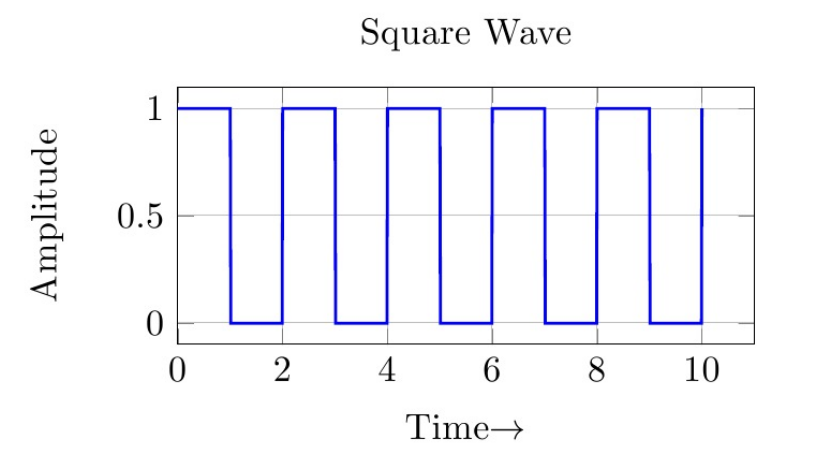
\includegraphics[width=\textwidth]{./imgs/Question-1-a.png}
		\caption{A square wave signal.}
	\end{figure}
\end{subquestion}

\begin{solution}
	In this case, we can see that our signal has a period of two, and hence $T = 2$. On the interval $[0, 2)$, we can therefore see that our signal $f(t)$ is given by:

	\begin{align*}
		f(t) &=
		\begin{cases}
			1, &0 \le t < 1 \\
			0, &1 \le t < 2
		\end{cases} \\
	\end{align*}

	Hence:

	\begin{align*}
		(f(t))^2 &=
		\begin{cases}
			1, &0 \le t < 1 \\
			0, &1 \le t < 2
		\end{cases}
	\end{align*}

	And so:

	\begin{align*}
		\int_{0}^{T}(f(t))^{2}dt &= \int_{0}^{1}(1)dt + \int_{1}^{2}(0)dt \\
		&= 1 + 0 \\
		&= 1 \\
	\end{align*}

	Thus, we have that the RMS of our signal is:

	\begin{align*}
		\sqrt{\frac{1}{T}\int_{0}^{T}(f(t))^{2}dt} &= \sqrt{\frac{1}{2}(1)} \\
		&= \sqrt{\frac{1}{2}} \\
		&= \frac{\sqrt{2}}{2} \\
	\end{align*}
\end{solution}

\begin{subquestion}
	Sawtooth Wave

	\begin{figure}[htbp]
		\centering
		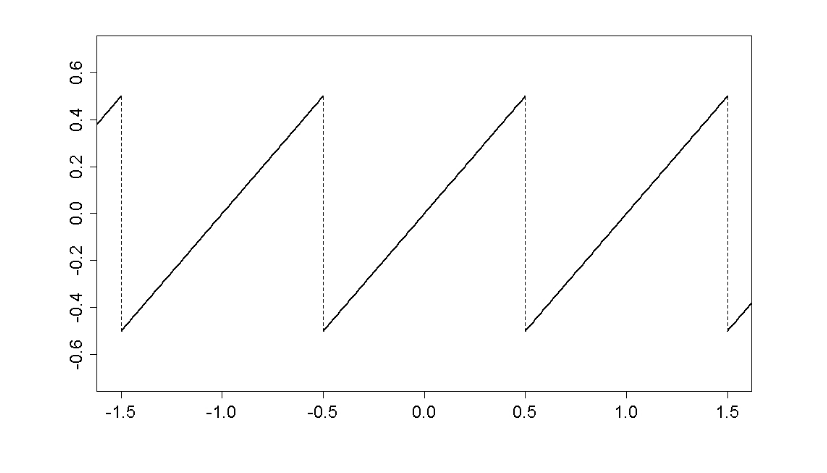
\includegraphics[width=\textwidth]{./imgs/Question-1-b.png}
		\caption{A sawtooth wave signal.}
	\end{figure}
\end{subquestion}

\begin{solution}
	We can now observe that our signal has a period of 1. On the interval $[0, 1)$, we can see that our signal $f(t)$ is given by:

	\begin{align*}
		f(t) &=
		\begin{cases}
			t, &0 \le t < \frac{1}{2} \\
			t - 1, &\frac{1}{2} \le t < 1
		\end{cases} \\
	\end{align*}

	Hence:

	\begin{align*}
		(f(t))^2 &=
		\begin{cases}
			t^2, &0 \le t < \frac{1}{2} \\
			(t - 1)^2, &\frac{1}{2} \le t < \frac{1}{2}
		\end{cases} \\
	\end{align*}

	And so:

	\begin{align*}
		\int_{0}^{T}(f(t))^{2}dt &= \int_{0}^{\frac{1}{2}}t^2{dt} + \int_{\frac{1}{2}}^{1}(t - 1)^2{dt} \\
		&= \int_{0}^{\frac{1}{2}}t^2{dt} + \int_{\frac{1}{2}}^{1}t^2 - 2t + 1{dt} \\
		&= \frac{1}{3}t^3 \big{|}_{0}^{\frac{1}{2}} + \frac{1}{3}t^3\big{|}_{\frac{1}{2}}^{1} - t^2\big{|}_{\frac{1}{2}}^{1} + t\big{|}_{\frac{1}{2}}^{1} \\
		&= \frac{1}{3}\left(\frac{1}{2}\right)^3 - 0 + \frac{1}{3}(1)^3 - \frac{1}{3}\left( \frac{1}{2} \right)^3 - (1)^2 + \left( \frac{1}{2} \right)^2 + 1 - \frac{1}{2} \\
		&= \frac{1}{24} \\
	\end{align*}

	Thus, we have that the RMS of our signal is:

	\begin{align*}
		\sqrt{\frac{1}{T}\int_{0}^{T}(f(t))^{2}dt} &= \sqrt{\frac{1}{1}\frac{1}{24}} \\
		&= \sqrt{\frac{1}{24}} \\
		&= \frac{\sqrt{3}}{6}
	\end{align*}
\end{solution}

\begin{subquestion}
	A Sine Wave

	\begin{figure}[htbp]
		\centering
		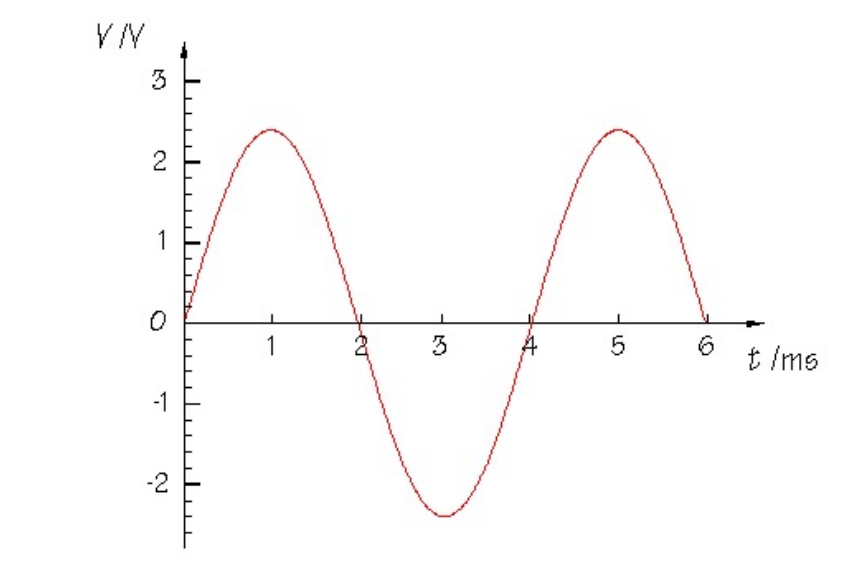
\includegraphics[width=\textwidth]{./imgs/Question-1-c.png}
		\caption{A sine wave signal.}
	\end{figure}
\end{subquestion}

\begin{solution}
	In this case, we can see that the sine wave has a period of 6 and an amplitude of $\frac{5}{2}$. This therefore implies that the frequency of the wave is given by $\omega = \frac{2\pi}{6} = \frac{\pi}{3}$. \\

	Hence, using the formula given in the question, we have that the wave's RMS is:

	\begin{align*}
		\sqrt{\frac{1}{T}\int_{0}^{T}(f(t))^{2}dt} &= \frac{B}{\sqrt{2}} \\
		&= \frac{5}{2\sqrt{2}} \\
		&= \frac{5\sqrt{2}}{4}
	\end{align*}
\end{solution}

\begin{question}
	Find the cut-off frequency of the following low-pass filters.
\end{question}

\begin{subquestion}
	Bode Plot 1.

	\begin{figure}[htbp]
		\centering
		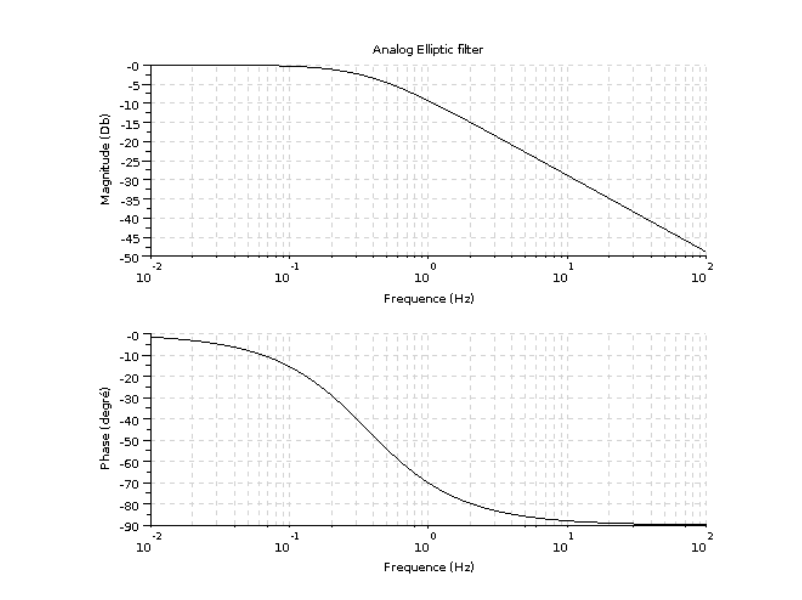
\includegraphics[width=\textwidth]{./imgs/Question-2-a.png}
		\caption{The first Bode plot.}
	\end{figure}
\end{subquestion}

\begin{solution}
	The cut-off frequency of a low-pass filter is the frequency at which the signal the output signal power drops to half the input signal power. This occurs when the filter's plotted magnitude decreases by 3dB. Hence, we can see that occurs approximately at a frequency of $10^{-\frac{1}{2}}$.
\end{solution}

\begin{subquestion}
	Bode Plot 2.

	\begin{figure}[htbp]
		\centering
		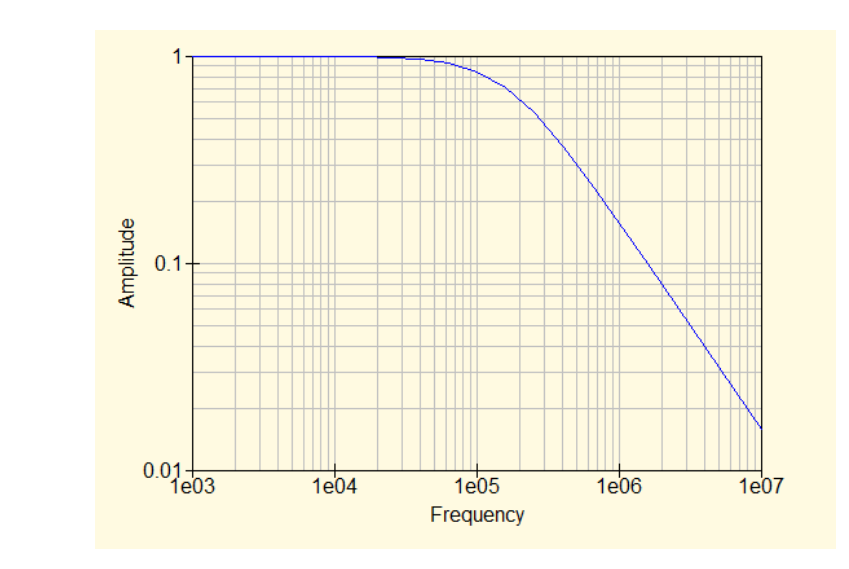
\includegraphics[width=\textwidth]{./imgs/Question-2-b.png}
		\caption{The second Bode plot.}
	\end{figure}
\end{subquestion}

\begin{solution}
	Here, the cutoff frequency corresponds to the frequency which has a value of $\sqrt{2}{2}$ of the signal's initial amplitude. This occurs at approximately a frequency of $3\cdot 10^{5}$.
\end{solution}

\begin{subquestion}
	Bode Plot 3.

	\begin{figure}[htbp]
		\centering
		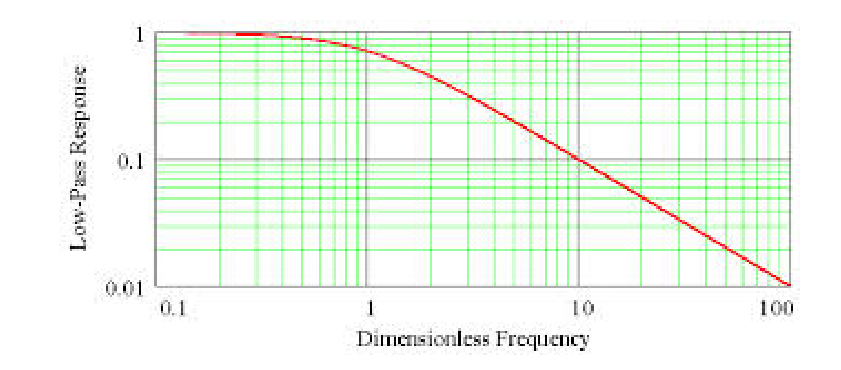
\includegraphics[width=\textwidth]{./imgs/Question-2-c.png}
		\caption{The last Bode plot.}
	\end{figure}
\end{subquestion}

\begin{solution}
	The low-pass response of a filter corresponds to its magnitude and so. However, this graph gives the low-pass response on a scale from 0-1, meaning a 3 dB drop corresponds to the frequency with a magnitude of $\sqrt{2}{2}$ of the initial magnitude, much as in the previous example. Thus we can see, looking at the graph, that its cutoff frequency is at a frequency of approximately 1.
\end{solution}

\end{document}
